% Latex file for the MPI Course at HPC2N Umea 
%    Elaborated by P. Ojeda
%
\documentclass{beamer}
%\documentclass[12pt]{article}
%\usepackage{beamerarticle}
\setbeamertemplate{navigation symbols}{}


\usetheme{Warsaw}
\usepackage{xcolor}
%\usepackage{chemmacros}
\usepackage{textpos}
%\usepackage{verbatim}
\usepackage{fancyvrb}
\DefineVerbatimEnvironment{ColorVerbatim}{Verbatim}%
  {formatcom=\color{purple},commandchars=\\\{\}}

%\usepackage[utf8]{inputenc}
%\usepackage[T1]{fontenc}
%\usepackage{lmodern}
\usepackage{listings}
%\usepackage{alltt}

\lstset{language=C,
  basicstyle=\ttfamily,
  keywordstyle=\color{blue}\ttfamily,
  stringstyle=\color{red}\ttfamily,
  commentstyle=\color{teal}\ttfamily,
  morecomment=[l][\color{magenta}]{\#}
}


\newcommand{\hilite}[1]{\colorbox{yellow}{#1}}

\setbeamercovered{invisible}
\beamersetuncovermixins{\opaqueness<1>{25}}{\opaqueness<2->{15}}
\begin{document}
% logo of my university
%\titlegraphic{\vspace*{-5cm} \hspace*{8.75cm} 
\includegraphics[width=1.5cm]{umea_logo.eps}
%}
%\logo{
\includegraphics[width=1.5cm]{umea_logo.eps}
%}

\title{ Introductory Course to Linux} \author{Pedro Ojeda-May, Birgitte Bryds\"{o}, and Jerry Eriksson
} \institute[Ume\aa University]{
  HPC2N, \\
  Ume\aa University,\\[1em]
\includegraphics[width=0.8cm]{images/umea_logo.eps} \\
  901 87, Sweden.
  }

%\date{September 17, 2018}
\date{}

% position the logo
\addtobeamertemplate{frametitle}{}{%
\begin{textblock*}{100mm}(\textwidth,-1.6cm)

\includegraphics[height=1cm,width=1cm,keepaspectratio]{images/logo_hpc2n.eps}
\end{textblock*}}

%%%%%%%%%%%%%%%%% NEW  SLIDE
\begin{frame}
	\titlepage
\end{frame}

%%%%%%%%%%%%%%%%% NEW  SLIDE
\begin{frame}
	\frametitle{Table of contents}

	\tableofcontents
\end{frame}



%########################  NEW SECTION  ########################
%% Section: Why?
% Latex file for the MPI Course at HPC2N Umea 
%    Elaborated by P. Ojeda
%

%########################  NEW SECTION  ########################
\section{Why?}



%%%%%%%%%%%%%%%%% NEW  SLIDE
\begin{frame}
	\frametitle{Why?}
  
	\begin{itemize}
		\item	Computations take too long time
			\begin{itemize}
				\item	Use an already parallelized software
				\item	Doing it yourself
					\begin{itemize}
						\item	Doing it yourself\\
								- Run each instance on a separate core\\
								- If inside a loop, maybe suitable for
										simple parallelization
						\item	More complex problems requires more explicit
								parallel programming
					\end{itemize}
			\end{itemize}
		\item	Use your computer for other things
		\item	Requires a lot of memory (up to 256 GB main memory)
		\item	Solve larger (more interesting/realistic) problems
	\end{itemize}

\end{frame}




%########################  NEW SECTION  ########################
%% Section: How to Apply
% Latex file for the MPI Course at HPC2N Umea 
%    Elaborated by P. Ojeda
%

%########################  NEW SECTION  ########################
\section{How to apply}

%------------------  NEW SUBSECTION ------------------
\subsection{Projects}

%%%%%%%%%%%%%%%%% NEW  SLIDE
\begin{frame}[fragile]
	\frametitle{SUPR - SNIC User and Project Repository}
	\begin{enumerate}
		\item	Get a login at SUPR (\texttt{https://supr.snic.se/})
		\item	Create a proposal for a project \\
				{\small  (at least: Title, Abstract, Resource Usage, Classification, length of project (1-12 months), which resource(s) you wish to use, and the amount of core hours/month you need.)}
		\item	Get an account at HPC2N
	\end{enumerate}
  
\end{frame}

%%%%%%%%%%%%%%%%% NEW  SLIDE
\begin{frame}
	\frametitle{Small level requests}
  
	\begin{itemize}
		\item	Max 5000 core hours/month/resource (Abisko)
		\item	Can be submitted at any time (short abstract)
		\item	Applications handled locally at the SNIC centers
		\item	For small projects and new groups that want to
				gain experience in using HPC systems
		\item	The PI must be employed at a Swedish university
				(e.g., PhD student or higher)
	\end{itemize}

\end{frame}

%%%%%%%%%%%%%%%%% NEW  SLIDE
\begin{frame}
	\frametitle{Medium level requests}
  
	\begin{itemize}
		\item	Up to 160000 core hours/month/resource (Abisko)
		\item	Can be submitted at any time
		\item	Applications handled locally at the SNIC centers
				and assesses the feasibility of using the requested recourses
		\item	Evaluated once a month
		\item	The PI must be a senior scientist in Swedish academia
	\end{itemize}

\end{frame}

%%%%%%%%%%%%%%%%% NEW  SLIDE
\begin{frame}
	\frametitle{Large level requests}
  
	\begin{itemize}
		\item	Above the medium level (160000 on Abisko)
		\item	Calls for proposals for large level allocations
				are issued twice a year by SNAC
		\item	Applications are evaluated by SNAC and they also decides on the
				allocations, based on scientific merit, need for the resources,
				efficient use of the resources, and impact
		\item	The PI must be a senior scientist in Swedish academia
	\end{itemize}

\end{frame}


%------------------  NEW SUBSECTION ------------------
\subsection{Accounts}

\begin{frame}
	\frametitle{User Account}

	\begin{itemize}
		\item	Submit an account application using our online form
			\begin{itemize}
				\item	Name and affiliation
				\item	Which project you are taking part in (if any)
				\item	Choose a user name
			\end{itemize}
		\item	Print the final form twice
			\begin{itemize}
				\item	Sign and send one to us together with a copy of
						your passport (do NOT send by email)
				\item	Keep one (your initial password is on it)
			\end{itemize}

	\end{itemize}

\end{frame}




%########################  NEW SECTION  ########################
%% Section: Support
% Latex file for the MPI Course at HPC2N Umea 
%    Elaborated by P. Ojeda
%


%########################  NEW SECTION  ########################
\section{Support}
\begin{frame}
	\frametitle{User Support}

	\begin{itemize}
		\item	\texttt{www.hpc2n.umu.se}
			\begin{itemize}
				\item	Quick-start guides
				\item	How to access, compile, and submit
				\item	Installed software\\
						- Descriptions and how to use them at HPC2N
			\end{itemize}
		\item	\texttt{support@hpc2n.umu.se}
			\begin{itemize}
				\item	Problems
				\item	Requests
			\end{itemize}
	\end{itemize}

\end{frame}

\begin{frame}
	\frametitle{User Support}

\includegraphics[width=10.5cm]{images/web.png}

\end{frame}

\begin{frame}
	\frametitle{User Support}

	\begin{itemize}
		\item	Meetings with individuals or groups
			\begin{itemize}
				\item	To see how can HPC2N be of help
				\item	Help to get started
				\item	Help to parallelize
			\end{itemize}
		\item	HPC2N Think Tank - Open house
		\item	Courses (0.5 - 3 days)
			\begin{itemize}
				\item	Introduction on how to use our system
				\item	Parallel programming (MPI, OpenMP) Oct. 2016
				\item	Computational Chemistry, MD simulations Nov. 2016
			\end{itemize}
	\end{itemize}

\end{frame}




%########################  NEW SECTION  ########################
% Section: Using Abisko
% Latex file for the MPI Course at HPC2N Umea 
%    Elaborated by P. Ojeda
%

%########################  NEW SECTION  ########################
\section{Linux}

%%%%%%%%%%%%%%%%% NEW  SLIDE
\begin{frame}
	\frametitle{Linux OS}
	
        \begin{center}
        \includegraphics[width=6.0cm]{images/linux_os.png}
        {\small Linux OS components.}
        \end{center}
\end{frame}

%%%%%%%%%%%%%%%%% NEW  SLIDE
\begin{frame}
	\frametitle{Linux }
	\begin{itemize}
		\item	UNIX-like OS 
		\item	used in modern Android smartphones
		\item   the difference between all UNIX-like OS is small	
	\end{itemize}
	
\end{frame}

%%%%%%%%%%%%%%%%%%%%%%%%%%%%%%%%%%%%%%%%%%%%%%%%%%%%%%%%%%%%%%%%%%%%%%%%%%%%%%%%%%%%%
\begin{frame}
	\frametitle{Linux timeline}
        \begin{center}
        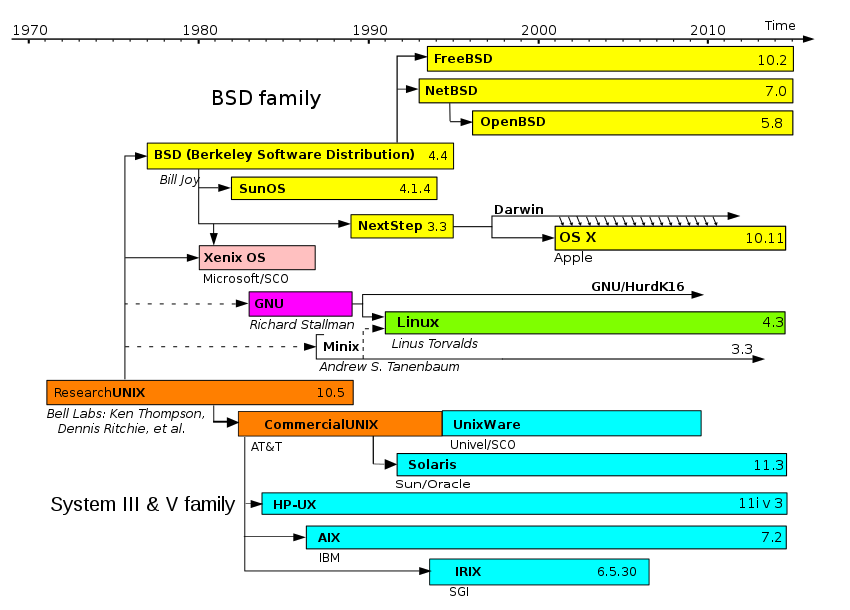
\includegraphics[width=8.0cm]{images/Unix_timeline.png}
        \end{center}
        {\tiny source: wikipedia}
\end{frame}

%%%%%%%%%%%%%%%%%%%%%%%%%%%%%%%%%%%%%%%%%%%%%%%%%%%%%%%%%%%%%%%%%%%%%%%%%%%%%%%%%%%%%
\begin{frame}
	\frametitle{The Linux terminal}
        \begin{center}
        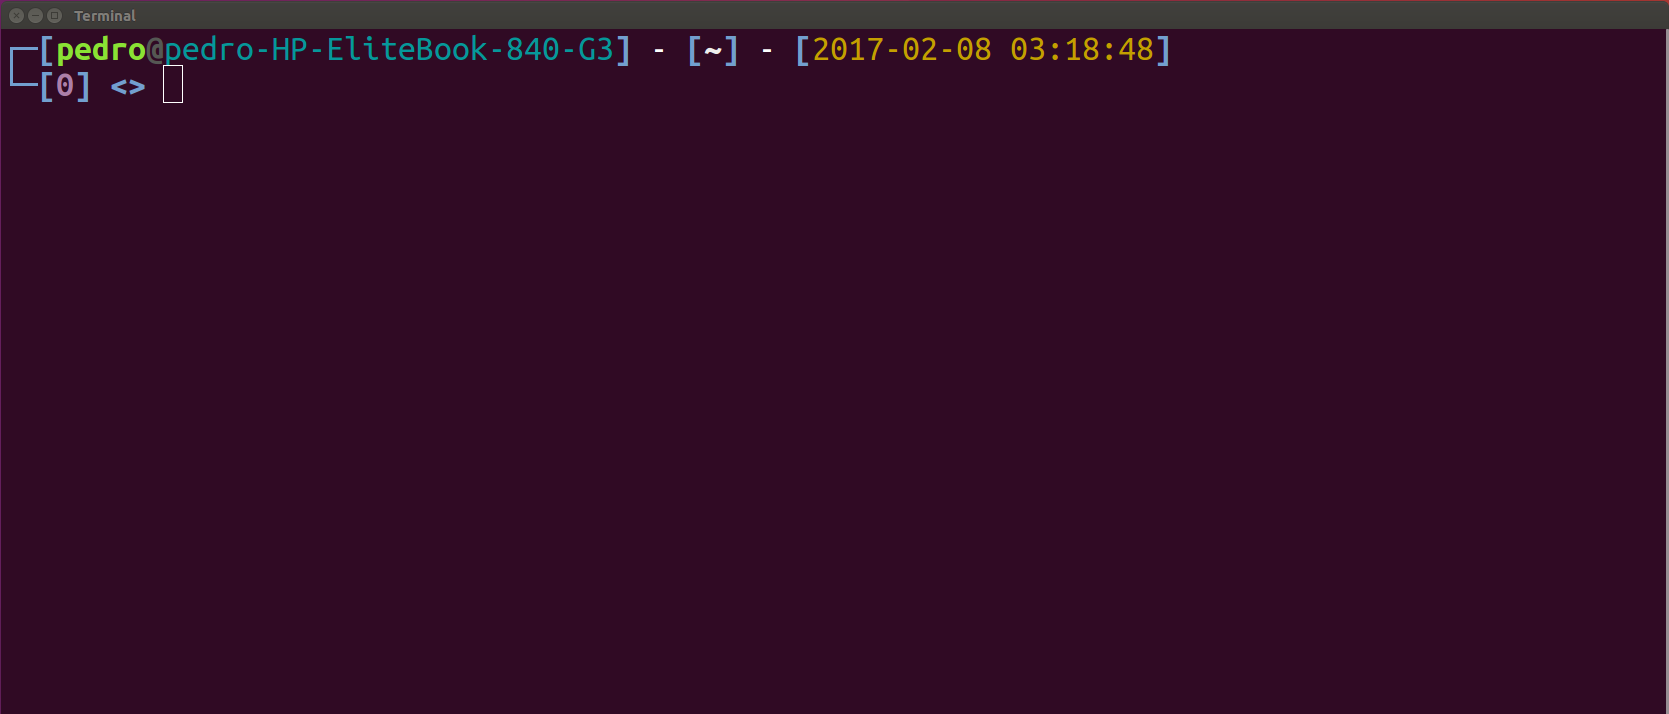
\includegraphics[width=9.5cm]{images/terminal_linux.png}
        \end{center}
	\begin{itemize}
		\item	on the terminal you can see the so-called Prompt
		\item	here you can control your PC/account or even
                 a remote server
	\end{itemize}
	
\end{frame}

%%%%%%%%%%%%%%%%%%%%%%%%%%%%%%%%%%%%%%%%%%%%%%%%%%%%%%%%%%%%%%%%%%%%%%%%%%%%%%%%%%%%%
\begin{frame}
	\frametitle{Files organization}
        \begin{center}
        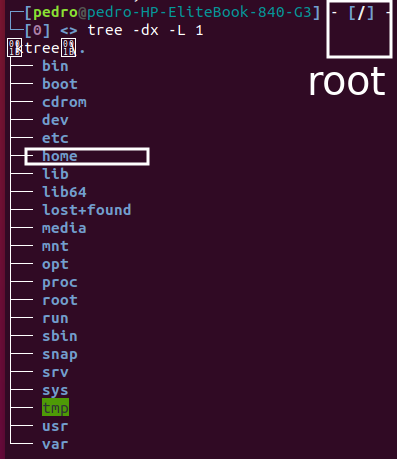
\includegraphics[width=7.5cm]{images/tree_root.png}
        \end{center}
\end{frame}
%%%%%%%%%%%%%%%%%%%%%%%%%%%%%%%%%%%%%%%%%%%%%%%%%%%%%%%%%%%%%%%%%%%%%%%%%%%%%%%%%%%%%
\begin{frame}
	\frametitle{Files organization}
        \begin{center}
        \includegraphics[width=10cm]{images/tree_organization.png}
        \end{center}
\end{frame}

%%%%%%%%%%%%%%%%%%%%%%%%%%%%%%%%%%%%%%%%%%%%%%%%%%%%%%%%%%%%%%%%%%%%%%%%%%%%%%%%%%%%%
\begin{frame}[fragile]
	\frametitle{ man}
        Manual pages. 
       
	\begin{itemize}
		\item \textbf{man command: man nano}
	\end{itemize}

{\tiny
	\begin{verbatim}
NANO(1)                     General Commands Manual                    NANO(1)

NAME
       nano - Nano's ANOther editor, an enhanced free Pico clone

SYNOPSIS
       nano [options] [[+line,column] file]...

DESCRIPTION
       nano  is  a small, free and friendly editor which aims to replace Pico,
       the default editor included in the non-free Pine package.   On  top  of
       copying  Pico's  look  and  feel, nano also implements some missing (or
       disabled by default) features in Pico, such as "search and replace" and
       "go to line and column number".
	\end{verbatim}
}
\end{frame}
%%%%%%%%%%%%%%%%%%%%%%%%%%%%%%%%%%%%%%%%%%%%%%%%%%%%%%%%%%%%%%%%%%%%%%%%%%%%%%%%%%%%%
\section{Navigating the File System}
\begin{frame}[fragile]
	\frametitle{}
\begin{center}
{\Huge
Navigating the File System
}
\end{center}

\end{frame}

%%%%%%%%%%%%%%%%%%%%%%%%%%%%%%%%%%%%%%%%%%%%%%%%%%%%%%%%%%%%%%%%%%%%%%%%%%%%%%%%%%%%%
\begin{frame}[fragile]
	\frametitle{ls}
List the content of a directory
{\scriptsize
	\begin{verbatim}
$ls
1CD9

$ls -l
total 24843644
drwxrwxr-x  2 pedro pedro        4096 nov  9 11:17 1CD9

$ls -la
total 24844368
drwxr-xr-x 44 pedro pedro        4096 feb 13 13:19 .
drwxr-xr-x  3 root  root         4096 sep 19 11:05 ..
drwxrwxr-x  2 pedro pedro        4096 nov  9 11:17 1CD9

$ls -lah
total 24G
drwxr-xr-x 44 pedro pedro 4,0K feb 13 13:25 .
drwxr-xr-x  3 root  root  4,0K sep 19 11:05 ..
drwxrwxr-x  2 pedro pedro 4,0K nov  9 11:17 1CD9
	\end{verbatim}
}

\end{frame}
%%%%%%%%%%%%%%%%%%%%%%%%%%%%%%%%%%%%%%%%%%%%%%%%%%%%%%%%%%%%%%%%%%%%%%%%%%%%%%%%%%%%%
\begin{frame}[fragile]
	\frametitle{ ls}
{\scriptsize
	\begin{verbatim}
$ls -laht
total 24G
drwxr-xr-x 44 pedro pedro 4,0K feb 13 13:29 .
-rw-------  1 pedro pedro 431K feb 13 13:29 .zsh_history
drwx------  6 pedro pedro 4,0K feb 13 13:28 Linux_Abisko_Kebne

$ls -lahrt
total 24G
-rw-r--r--  1 pedro pedro  655 sep 19 11:05 .profile
	\end{verbatim}
}

\end{frame}
%%%%%%%%%%%%%%%%%%%%%%%%%%%%%%%%%%%%%%%%%%%%%%%%%%%%%%%%%%%%%%%%%%%%%%%%%%%%%%%%%%%%%
\begin{frame}[fragile]
	\frametitle{ chmod}
Change permissions.

Useful cases:
	\begin{itemize}
        \item chmod Y+Z 
        \item Y=u,g,o 
        \item Z=r,w,x
	\end{itemize}
        
\end{frame}

%%%%%%%%%%%%%%%%%%%%%%%%%%%%%%%%%%%%%%%%%%%%%%%%%%%%%%%%%%%%%%%%%%%%%%%%%%%%%%%%%%%%%
\begin{frame}[fragile]
	\frametitle{ cd}
Change directory.

Useful cases:
	\begin{itemize}
        \item cd directory 

        move to "directory" 
        \item cd
 
         move to $\$HOME$ directory
        \item cd - 

        move to previous visited directory

        \item cd ..

        move to upper directory in the hierarchical tree

        \item pwd 
        prints out the local directory path
 
	\end{itemize}
        
\end{frame}

%%%%%%%%%%%%%%%%%%%%%%%%%%%%%%%%%%%%%%%%%%%%%%%%%%%%%%%%%%%%%%%%%%%%%%%%%%%%%%%%%%%%%
\begin{frame}
	\frametitle{ cp}
        Copy files.

Useful cases:
	\begin{itemize}
        \item cp text.txt directory/

        copy text.txt file to "directory" 
        \item cp -r test/ directory/ 
 
        copy the directory test into directory/. 

        cp overwrites existing files!

	\end{itemize}
        

\end{frame}


%%%%%%%%%%%%%%%%%%%%%%%%%%%%%%%%%%%%%%%%%%%%%%%%%%%%%%%%%%%%%%%%%%%%%%%%%%%%%%%%%%%%%
\begin{frame}
	\frametitle{ touch/mkdir}
        Create files.

Useful cases:
	\begin{itemize}
        \item touch text.txt

        creates text.txt file  
        \item mkdir test  
 
        creates the directory test 

	\end{itemize}

\end{frame}

%%%%%%%%%%%%%%%%%%%%%%%%%%%%%%%%%%%%%%%%%%%%%%%%%%%%%%%%%%%%%%%%%%%%%%%%%%%%%%%%%%%%%
\begin{frame}
	\frametitle{ rm}
        Remove files.

Useful cases:
	\begin{itemize}
        \item rm text.txt

        deletes text.txt file  
        \item rm -rf test/  
 
        deletes the directory test 

        deleted files cannot be recovered!

	\end{itemize}
        

\end{frame}

%%%%%%%%%%%%%%%%%%%%%%%%%%%%%%%%%%%%%%%%%%%%%%%%%%%%%%%%%%%%%%%%%%%%%%%%%%%%%%%%%%%%%
\begin{frame}
	\frametitle{Wild cards}

	\begin{itemize}
        \item ?

        it represents a single character

        \item *

        it represents a string of characters
 
        \item $\left[0-9\right], \left[A-B\right]$

        it represents a range of numbers or characters
	\end{itemize}
        

\end{frame}
%%%%%%%%%%%%%%%%%%%%%%%%%%%%%%%%%%%%%%%%%%%%%%%%%%%%%%%%%%%%%%%%%%%%%%%%%%%%%%%%%%%%%
\begin{frame}[fragile]
	\frametitle{Symbolic links}

also called soft links is a pointer file to other file/directory. One can create
a soft link with the $ln$ command: 
        
\begin{verbatim}
ln -s source.txt link

ls -l source.txt link 
lrwxrwxrwx 1 pedro pedro 14 sep  8 22:14 link -> source.txt
-rw-r--r-- 1 pedro pedro  0 sep  8 22:13 source.txt
\end{verbatim}


\end{frame}
%%%%%%%%%%%%%%%%%%%%%%%%%%%%%%%%%%%%%%%%%%%%%%%%%%%%%%%%%%%%%%%%%%%%%%%%%%%%%%%%%%%%%
\begin{frame}[fragile]
	\frametitle{Redirection}

       
we can change the standard input (keyboard)/output (screen) of Linux commands:
 

\begin{itemize}
   \item The operator $>$ redirects the output of some command 

   $ls > test.dat$

   in this case to the file test.dat

   \item The operator $>>$ concatenate the output of some command to the content 
   of a file:

   $ls >> test.dat$

   \item The operator $<$ changes the standard input

   \item The operator $2>$ redirects the standard error:

   $exec 2>error.log$

   \item The operator $2>\&1$, redirects both standard output and error:
   $exec > logfile  2>\&1$
\end{itemize}


\end{frame}
%%%%%%%%%%%%%%%%%%%%%%%%%%%%%%%%%%%%%%%%%%%%%%%%%%%%%%%%%%%%%%%%%%%%%%%%%%%%%%%%%%%%%
\begin{frame}[fragile]
	\frametitle{Pipes}
	\begin{itemize}
         \item  One can use the output of some command as the input for another command:
	\end{itemize}

\begin{verbatim}
grep 'string' file.txt | wc 
grep 'string' file.txt > file.out
grep 'string' file.txt >> file.out
\end{verbatim}

\end{frame}
%%%%%%%%%%%%%%%%%%%%%%%%%%%%%%%%%%%%%%%%%%%%%%%%%%%%%%%%%%%%%%%%%%%%%%%%%%%%%%%%%%%%%
\begin{frame}[fragile]
	\frametitle{Exporting variables}

\begin{itemize}
   \item some programs or libraries require environment variables to work
   \item they allow the program to follow different schemes without being re-compiled
   \item some variables such as $\$HOME$ are intrinsic to Linux OS
   \item we need to export the variables for further use:

\begin{verbatim}
$export NUMBER_OF_THREADS=6
\end{verbatim}
\end{itemize}

\end{frame}
%%%%%%%%%%%%%%%%%%%%%%%%%%%%%%%%%%%%%%%%%%%%%%%%%%%%%%%%%%%%%%%%%%%%%%%%%%%%%%%%%%%%%
\begin{frame}
	\frametitle{Editing files}
        \begin{center}
        \includegraphics[width=10cm]{images/nano.png}
        \end{center}
\end{frame}

%%%%%%%%%%%%%%%%%%%%%%%%%%%%%%%%%%%%%%%%%%%%%%%%%%%%%%%%%%%%%%%%%%%%%%%%%%%%%%%%%%%%%
\section{Data Handling}
\begin{frame}[fragile]
	\frametitle{}
\begin{center}
{\Huge
Data Handling
}
\end{center}

\end{frame}


%%%%%%%%%%%%%%%%%%%%%%%%%%%%%%%%%%%%%%%%%%%%%%%%%%%%%%%%%%%%%%%%%%%%%%%%%%%%%%%%%%%%%
\begin{frame}[fragile]
	\frametitle{Compress/decompress files}

Compressing files:

\begin{verbatim}
$gzip file     --->  file.gz
\end{verbatim}

Decompressing files:

\begin{verbatim}
$gunzip file.gz
\end{verbatim}

\end{frame}

%%%%%%%%%%%%%%%%%%%%%%%%%%%%%%%%%%%%%%%%%%%%%%%%%%%%%%%%%%%%%%%%%%%%%%%%%%%%%%%%%%%%%

\begin{frame}[fragile]
	\frametitle{Generating archives}

Generate tar-ball:

\begin{verbatim}
$tar -cvf directory.tar directory 
\end{verbatim}

Opening tar-ball:

\begin{verbatim}
$tar -xvf directory.tar
\end{verbatim}

\end{frame}


%%%%%%%%%%%%%%%%%%%%%%%%%%%%%%%%%%%%%%%%%%%%%%%%%%%%%%%%%%%%%%%%%%%%%%%%%%%%%%%%%%%%%
\begin{frame}
	\frametitle{ ssh}
Command for connecting to a remote computer.

Useful cases:
	\begin{itemize}
         \item ssh username@abisko.hpc2n.umu.se

         connecting to abisko machine

         \item ssh -Xl username abisko.hpc2n.umu.se

        if you want to enable graphical display.

	\end{itemize}
\end{frame}

%%%%%%%%%%%%%%%%%%%%%%%%%%%%%%%%%%%%%%%%%%%%%%%%%%%%%%%%%%%%%%%%%%%%%%%%%%%%%%%%%%%%%
\begin{frame}[fragile]
	\frametitle{ sftp (scp)}

Protocol for data transfer.
\begin{verbatim}
$sftp username@abisko.hpc2n.umu.se

$get file

$put file

\end{verbatim}
\end{frame}

%%%%%%%%%%%%%%%%%%%%%%%%%%%%%%%%%%%%%%%%%%%%%%%%%%%%%%%%%%%%%%%%%%%%%%%%%%%%%%%%%%%%%
\begin{frame}[fragile]
	\frametitle{ rsync}

Protocol for synchronizing data.
\begin{verbatim}
rsync source target

rsync -az user@kebne.hpc2n.umu.se:/home/proj/ proj/
\end{verbatim}
\end{frame}


\section{Finding Patterns}
%%%%%%%%%%%%%%%%%%%%%%%%%%%%%%%%%%%%%%%%%%%%%%%%%%%%%%%%%%%%%%%%%%%%%%%%%%%%%%%%%%%%%
\begin{frame}[fragile]
	\frametitle{}
\begin{center}
{\Huge
Finding patterns
}
\end{center}

\end{frame}

%%%%%%%%%%%%%%%%%%%%%%%%%%%%%%%%%%%%%%%%%%%%%%%%%%%%%%%%%%%%%%%%%%%%%%%%%%%%%%%%%%%%%
\begin{frame}
	\frametitle{ grep}
      This command searches for patterns in text files.

Useful cases:
	\begin{itemize}
        \item grep 'word' file

        it searches for pattern 'word' in file

        \item grep -rine 'word' home

        pattern word is searched recursively in the directory  $/home$
 
	\end{itemize}

\end{frame}

%%%%%%%%%%%%%%%%%%%%%%%%%%%%%%%%%%%%%%%%%%%%%%%%%%%%%%%%%%%%%%%%%%%%%%%%%%%%%%%%%%%%%
\begin{frame}
	\frametitle{ awk}
This command finds patterns in a file and can perform arithmetic/string operations.

Useful cases:
	\begin{itemize}
        \item awk '/gold/ $\{print  \$1 \} $' file

        \item it searches for pattern 'gold' in file and prints out the first column 

	\end{itemize}

\end{frame}

%%%%%%%%%%%%%%%%%%%%%%%%%%%%%%%%%%%%%%%%%%%%%%%%%%%%%%%%%%%%%%%%%%%%%%%%%%%%%%%%%%%%%
\section{Scripting}
\begin{frame}[fragile]
	\frametitle{}
\begin{center}
{\Huge
Scripting
}
\end{center}

\end{frame}


\begin{frame}
	\frametitle{Scripting}

\begin{itemize}
\item allows to perform complex tasks without user intervention
\item all Linux commands can be used in a script including wild cards

\end{itemize}

\end{frame}
%%%%%%%%%%%%%%%%%%%%%%%%%%%%%%%%%%%%%%%%%%%%%%%%%%%%%%%%%%%%%%%%%%%%%%%%%%%%%%%%%%%%%

\begin{frame}[fragile]
	\frametitle{Scripting}

\begin{block}{analysis.sh}
\begin{verbatim}
#!/bin/bash

grep 'ABCD' file.pdb >  file_filtered.pdb 

program < file_filtered.pdb > output.dat

\end{verbatim}
\end{block}

execute script with ./analysis.sh

\end{frame}
%%%%%%%%%%%%%%%%%%%%%%%%%%%%%%%%%%%%%%%%%%%%%%%%%%%%%%%%%%%%%%%%%%%%%%%%%%%%%%%%%%%%%

\begin{frame}[fragile]
	\frametitle{Scripting}

\begin{verbatim}
$ls -lah
total 24G
drwxrwxr-x  2 pedro pedro 4,0K nov  9 11:17 1CD9
\end{verbatim}

\begin{itemize}
\item permissions are set of "user", "group", or "others"
\item we can change permissions with chmod command
\end{itemize}

For instance, 

\begin{verbatim}
$chmod u+x analysis.sh

$execute script with ./analysis.sh
\end{verbatim}

\end{frame}

%%%%%%%%%%%%%%%%%%%%%%%%%%%%%%%%%%%%%%%%%%%%%%%%%%%%%%%%%%%%%%%%%%%%%%%%%%%%%%%%%%%%%

\section{More advanced topics}

\begin{frame}[fragile]
	\frametitle{Working with the Prompt}

\begin{itemize}
\item ctrl+a:	Go to the beginning of the line
\item ctrl+e:	Go to the end of the line
\item ctrl+l:   Clean the terminal
\end{itemize}

\end{frame}

%%%%%%%%%%%%%%%%%%%%%%%%%%%%%%%%%%%%%%%%%%%%%%%%%%%%%%%%%%%%%%%%%%%%%%%%%%%%%%%%%%%%%
\begin{frame}[fragile]
	\frametitle{Configuring .bashrc file}

Exploring the history:

by typing "ctrl+r" you will be prompted to introduce text which bash 
will use to make a search in the list of commands you have typed previously.
That list is saved in the .bash\_history file in your home directory.  

One can control the behavior of the history file by setting environment variables
in the .bashrc file as follows:

\begin{verbatim}
export HISTCONTROL=erasedups
export HISTSIZE=100000
export HISTFILESIZE=100000
shopt -s histappend
\end{verbatim}


\end{frame}
%%%%%%%%%%%%%%%%%%%%%%%%%%%%%%%%%%%%%%%%%%%%%%%%%%%%%%%%%%%%%%%%%%%%%%%%%%%%%%%%%%%%%
\begin{frame}[fragile]
	\frametitle{Configuring .bashrc file}

Using aliases:

if you need to type a long command several times, you may add it as an alias in 
your .bashrc file:

\begin{verbatim}
alias ldir='ls -lahrt | egrep "^d"'
\end{verbatim}

\end{frame}
%%%%%%%%%%%%%%%%%%%%%%%%%%%%%%%%%%%%%%%%%%%%%%%%%%%%%%%%%%%%%%%%%%%%%%%%%%%%%%%%%%%%%
\begin{frame}[fragile]
	\frametitle{Specific commands on our cluster}

\begin{itemize}
\item projinfo: information of the usage of the project resources
\item squeue -a -u username: status of the jobs for username
\item sbatch script.sh: for job submission
\item scancel jobid: for cancelling a job
\item quota: information of the /home and /pfs disk usage
\end{itemize}

\end{frame}
%%%%%%%%%%%%%%%%%%%%%%%%%%%%%%%%%%%%%%%%%%%%%%%%%%%%%%%%%%%%%%%%%%%%%%%%%%%%%%%%%%%%%

\begin{frame}
	\frametitle{Linux Cheat Sheet}

\begin{itemize}
\item https://www.hpc2n.umu.se/documentation/guides/linux-cheat-sheet
\end{itemize}

\end{frame}


%########################  NEW SECTION  ########################
%% Section: Using Abisko
% Latex file for the MPI Course at HPC2N Umea 
%    Elaborated by P. Ojeda
%

%########################  NEW SECTION  ########################
\section{Using Abisko}

%%%%%%%%%%%%%%%%% NEW  SLIDE
\begin{frame}
	\frametitle{Abisko}
\includegraphics[width=4.5cm]{images/kebnekeise.eps}
	\begin{itemize}
		\item	332 nodes/15936 cores
		\item	10 fat nodes (512 GB RAM), 318 thin nodes (128 GB RAM)
		\item	CPUs: (thin) 4 x AMD Opteron 6238 (Interlagos) 12 core (2.6 GHz)
		\item	CPUs: (fat) 4 x AMD Opteron 6344 (Abu Dhabi) 12 core (2.6 GHz)
		\item	Interconnect: Infiniband QDR, 40Gb/s, Mellanox
		\item	Installed 2011
	\end{itemize}
\end{frame}




%########################  NEW SECTION  ########################
%% Section: Hands On
% Latex file for the MPI Course at HPC2N Umea 
%    Elaborated by P. Ojeda
%

%########################  NEW SECTION  ########################
\section{Hands-on}



%%%%%%%%%%%%%%%%% NEW  SLIDE
\begin{frame}
	\frametitle{Simple hands-on}
  
	\begin{enumerate}
		\item	Log in to Abisko.
		\item	Go to the parallel file system.
		\item	Copy executable (threaded program)and submit file:\\
				\texttt{cp \~{}mr/Public/mandel .}\\
				\texttt{cp \~{}mr/Public/submit .}
		\item	Put the submit file into the batch queue.
		\item	Look at the queue.
		\item	Where did the output from the program go?
		\item	Run on 12 cores instead.
				Does it run twice as fast?
		\item	The program creates a picture on a file (\texttt{mandel.ppm})
				as output.
				Try looking at it (e.g. using the command \texttt{display}).
	\end{enumerate}

\end{frame}





\end{document}
